% this document is part of the DoCrimes project.
% Copyright 2022 the authors

\documentclass[modern]{aastex631}
\usepackage[utf8]{inputenc}

% typesetting issues
\setlength{\parindent}{3.5ex}
\sloppy\sloppypar\raggedbottom\frenchspacing
\renewcommand{\twocolumngrid}{} % oh yes I can do that

% figure issues
\usepackage[framemethod=tikz]{mdframed}
\usetikzlibrary{shadows}
\definecolor{captiongray}{HTML}{555555}
\mdfsetup{%
  innertopmargin=2ex,
  innerbottommargin=1.8ex,
  linecolor=captiongray,
  linewidth=0.5pt,
  roundcorner=5pt,
  shadow=true,
  shadowcolor=black!05,
  shadowsize=4pt
}
\newlength{\widefigurewidth}
\setlength{\widefigurewidth}{0.95\textwidth}
\newlength{\figurewidth}
\setlength{\figurewidth}{0.75\textwidth}

% math definitions
\newcommand{\unit}[1]{\mathrm{#1}}
\newcommand{\Gpc}{\unit{Gpc}}
\newcommand{\mg}{\unit{mag}}

% text definitions
\shortauthors{hogg and storey-fisher}
\shorttitle{testing isotropy and homogeneity}
\newcommand{\documentname}{\textsl{Article}}
\newcommand{\figref}[1]{\figurename~\ref{#1}}

\begin{document}

\title{%
Testing cosmic isotropy and homogeneity
with \textsl{Gaia} quasars}
\author[0000-0003-2866-9403]{David W. Hogg}
\affil{Center for Cosmology and Particle Physics, Department of Physics, New York University}
\affil{Max-Planck-Institut f\"ur Astronomie}
\affil{Flatiron Institute, a division of the Simons Foundation}

\author[0000-0001-8764-7103]{Kate Storey-Fisher}
\affil{Center for Cosmology and Particle Physics, Department of Physics, New York University}

\date{2022 August}

\begin{abstract}\noindent
All cosmological models in general relativity are built on the assumption of large-scale isotropy and homogeneity.
These assumptions are testable.
Tests of cosmic isotropy and homogeneity are also strong tests of the quality of data or catalogs and their calibration.
Test precision increases as observations cover more solid angle, become more sensitive to distant objects, and are made with more uniform data.
The ESA \textsl{Gaia} Mission is primarily concerned with stars in the Milky Way, but it also observes millions of quasars, all sky (modulo Galactic extinction), to redshifts of around $4.5$.
It has produced the largest-comoving-volume public quasar catalog to date.
Here we use a carefully curated subsample of ZZZ \textsl{Gaia} quasars to show that the angular distribution, redshift distribution as a function of sky position, amplitude of clustering as a function of sky position, and counts of pairs as a function of separation (fractal dimension), are all consistent with large-scale isotropy and homogeneity at the precision possible given the size of the catalog and the amplitude of the large-scale structure.
Roughly speaking, the results can be summarized by saying that they show the Universe to be isotropic to better than XXX percent and homogeneous to better than YYY percent.
There is no sign of any North--South power asymmetry.
The isotropy results can also be interpreted as a strong test of the spectrophotometric uniformity of the \textsl{Gaia} Catalog.
\end{abstract}

\keywords{%
calibration
---
catalogs
---
cosmic~isotropy
---
cosmological~principle
---
cosmology
---
large-scale~structure~of~the~Universe
---
quasars
}
\section*{}
\clearpage
\section{Introduction}

One of the fundamental assumptions of the physical cosmological model is that the Universe is isotropic and homogeneous on large scales (CITE).
This assumption is testable.
It is worthy of test, both because it is always worth testing fundamental assumptions, and because the large-scale structure has self-similar or fractal characteristics (CITE), which are characteristic of inhomogeneous distributions.
And, even in the ascendent physical model of cosmology, there is expected to be at least some power in the initial conditions on all length scale (CITE).

If the Universe failed tests of homogeneity on large scales, and in particular if the Universe turned out to be a fractal with a fractal dimension significantly less than 3, we would be in big trouble theoretically.
Why?
Because a fractal universe has no well-defined mean density.
There are no working physical models for such an inhomogeneous universe.
Indeed, there are not even any known solutions of the equations of general relativity without a well-defined mean density.

All that said, we know now that the Universe is not a fractal on large scales (CITE).
There are other reasons to continue to test isotropy and homogeneity however.
One is that the cosmic microwave background appears to show a power asymmetry, in which there appears to be a larger amplitude of fluctuations in the North/South Galactic Cap than there is in the South/North (CITE).
If this asymmetry is real, it should show itself in the large-scale structure as well (CITE).

Another reason to make new tests of isotropy and homogeneity is that data samples keep getting larger in volume and number, permitting more and more sensitive tests.
Here we make use of the brand-new ESA \textsl{Gaia} DR3 data (CITE), which includes hundreds of thousands or even millions of quasars, all-sky (CITE).
This data set is not the largest cosmological data set in terms of number of tracers, but it is the largest-ever data set in terms of comoving volume, spanning some XXX $h^{-3}\,\Gpc^3$ (comoving), depending on how you want to define the sample volume.

A final but equally important reason to test isotropy and homogeneity is that these tests provide a very strong validation of the quality and uniformity of the data.
Indeed, the first work on homogeneity with the Sloan Digital Sky Survey data (CITE) was performed to test the calibration and stability of the data in preparation for the measurement of the baryon acoustic feature (CITE).
The work presented here represents a first strong test of the calibration and isotropy of the \textsl{Gaia} quasar sample.

\section{Data}

Hogg say: Make sure we cite the CU5 papers here and anything that helped make the extragalactic and quasar samples.

The data used in this project is the XXX quasar sample (\citealt{ksf}), derived from the ESA \textsl{Gaia} quasar candidate catalog (CITE).
This candidate catalog was released as part of the \textsl{Gaia} Data Release 3 data (DR3; CITE).
The catalog was constructed using the overlap of the \textsl{Gaia} DR3 data with photometry from the NASA \textsl{WISE} Mission (CITE), and spectro-photometric redshifts were estimated using a combination of XXX photometry, \textsl{Gaia} DR3 \texttt{qsoc} (maybe?) redshift estimates, and a training set from \textsl{SDSS-IV} Data Release 17 data (CITE).
For more information see the XXX quasar catalog paper (\citealt{ksf}).

\begin{figure}[t!]
  \begin{mdframed}
  \color{captiongray}
  \begin{center}
    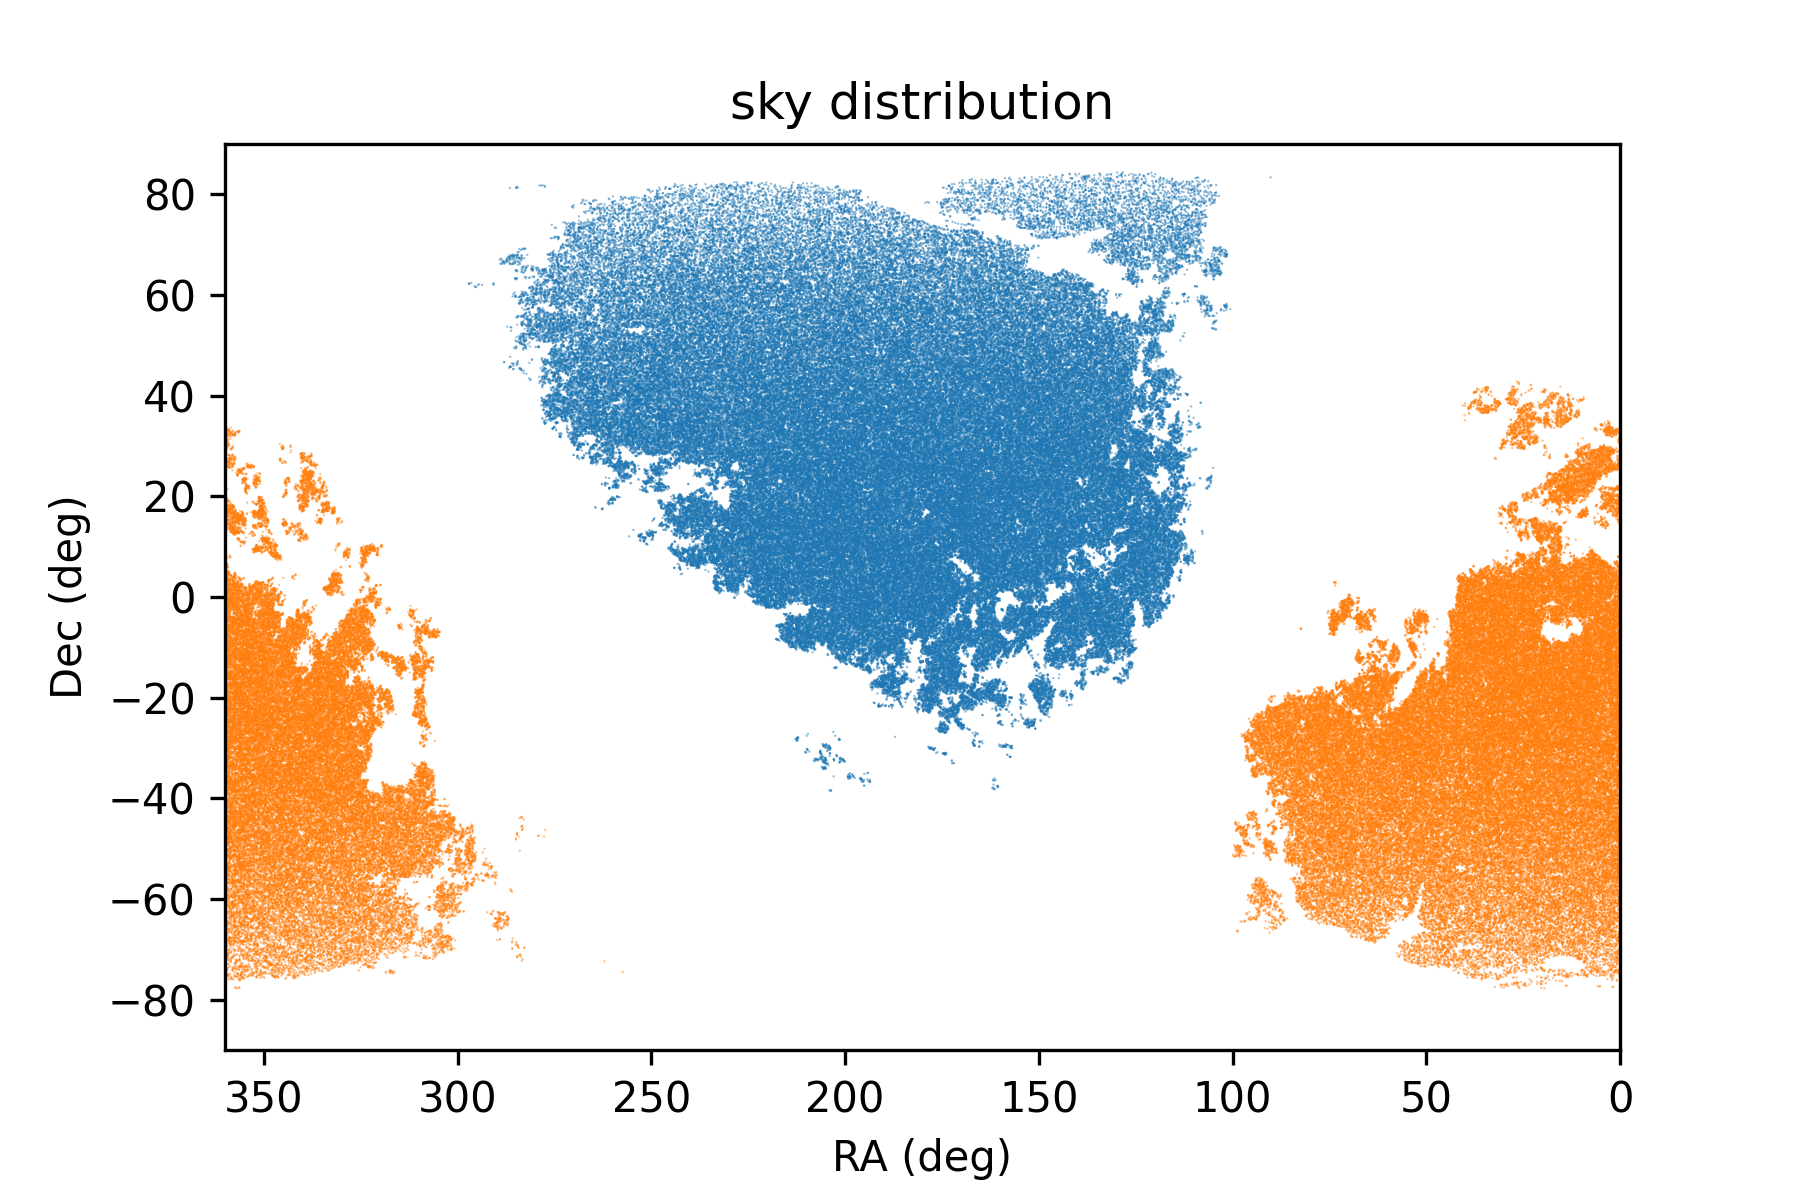
\includegraphics[width=\figurewidth]{notebooks/radec.png}
  \end{center}
    \caption{The full quasar sample, obtained after cutting on apparent magnitude and extinction, plotted on the sky in Equatorial coordinates.
    The NGC subsample (and its associated random catalog) is colored blue and the SGC subsample is colored orange.
    Stars from the Bright Star Catalog (\citealt{bsc}) with $V<4\,\mg$ are shown as grey disks for angular reference.\label{fig:radec}}
  \end{mdframed}
\end{figure}
We cut the full XXX quasar sample to \textsl{Gaia} $G<20\,\mg$ for redshift reliability.
We further cut it to an infrared-emission-based extinction estimate of YYYY$<$whatever (\citealt{sfd}) for angular uniformity.
Finally, we tag those quasars with Galactic latitude $b>0$ ``North Galactic Cap'' (NGC) and those with $b<0$ ``South Galactic Cap'' (SGC).
These cuts leave XXX quasars in the sample, YYY in the NGC subsample and ZZZ in the SGC subsample.
The sample is shown on the sky in the equatorial coordinate system in \figref{fig:radec}.

\begin{figure}[t!]
  \begin{mdframed}
  \color{captiongray}
  \begin{center}
    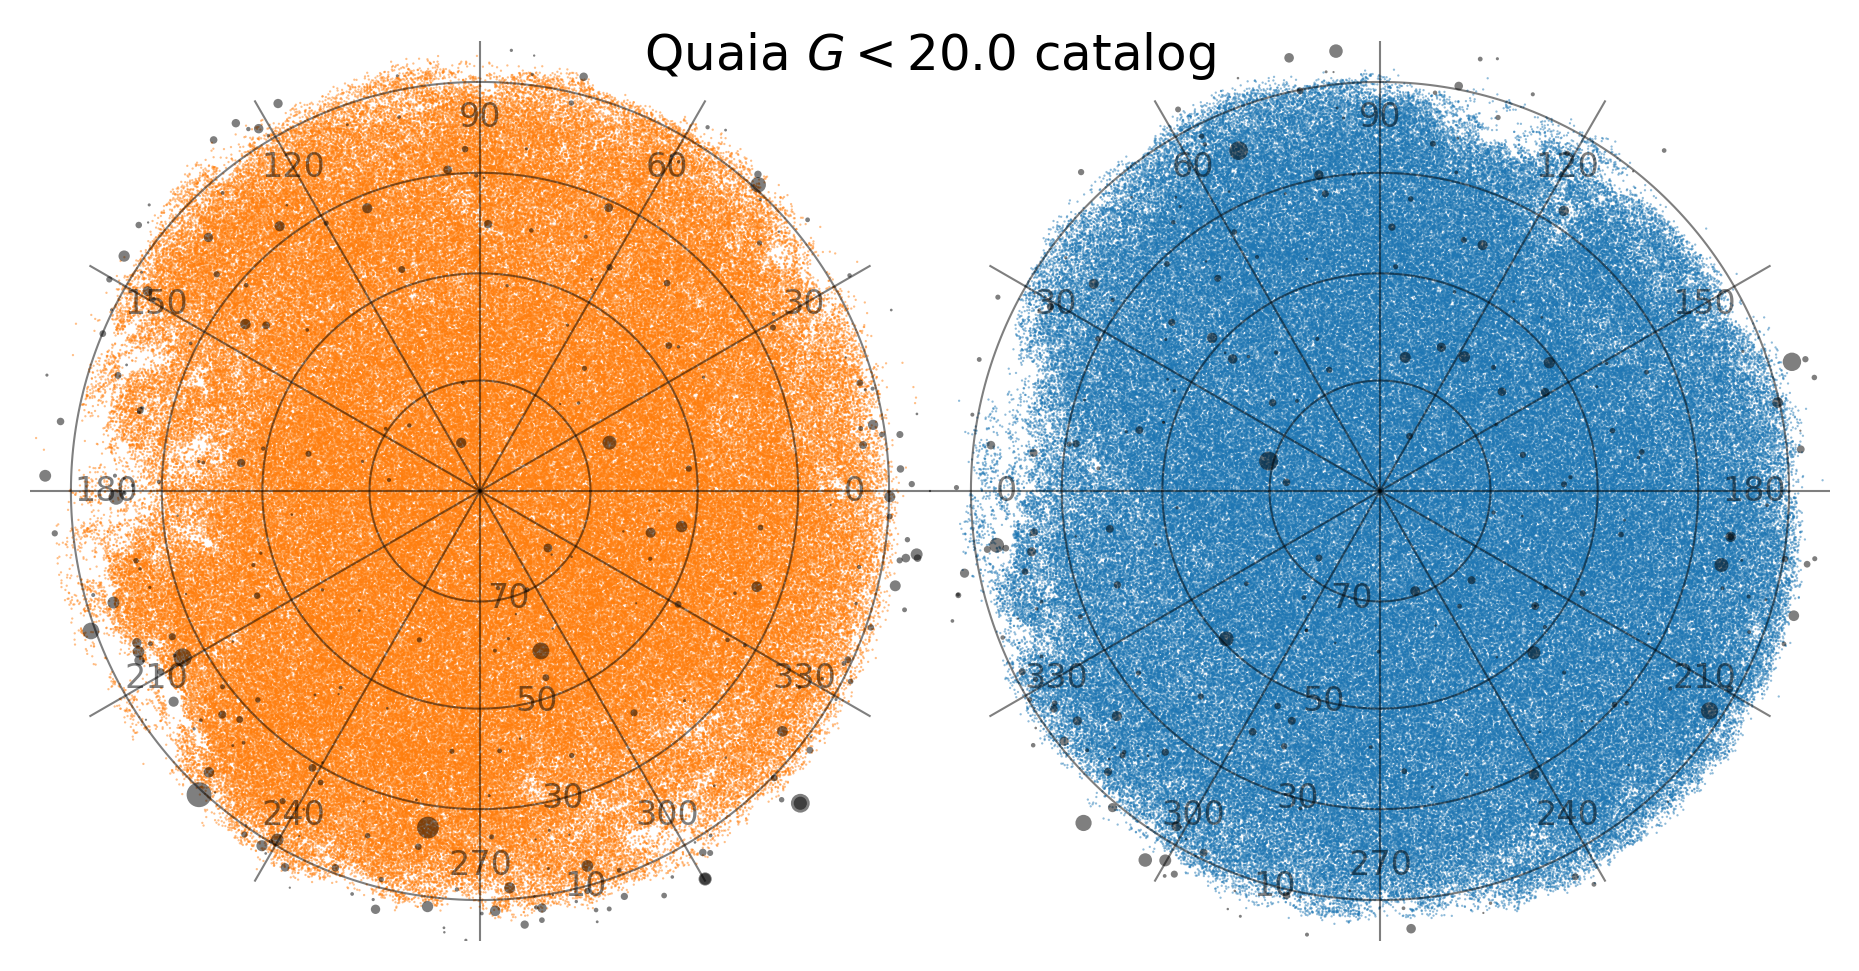
\includegraphics[width=\figurewidth]{notebooks/lb.png}\\
    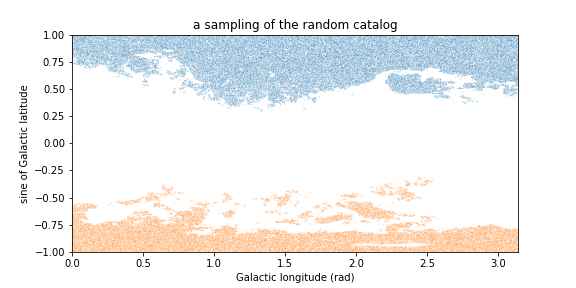
\includegraphics[width=\figurewidth]{notebooks/lb_random.png}
  \end{center}
    \caption{The full quasar sample obtained after cutting on apparent magnitude and extinction (top) and a sampling of the much larger random catalog obtained after making those same cuts (bottom), plotted on the sky in Galactic coordinates.
    This projection is designed to be equal-area (the Lambert azimuthal equal-area projection), such that a set of quasars uniformly distributed on the sky would make a set of points uniformly distributed on this 2-d plot.
    The NGC subsample (and its associated random catalog) is colored blue and the SGC subsample (and its associated random catalog) is colored orange.
    Stars from the Bright Star Catalog (\citealt{bsc}) with $V<4\,\mg$ are shown as grey disks for angular reference.\label{fig:lb}}
  \end{mdframed}
\end{figure}
The XXX quasar catalog comes with an associated random catalog with a near-identical sky footprint but YYYY times the density (\citealt{ksf}).
The random-catalog footprint is modulated by stellar density and Galactic extinction, with these modulations fit to match the observed data.
We cut the random catalog identically to the quasar catalog.
Both the quasar catalog and an equivalent-density sampling of the random catalog are shown on the sky in the Galactic coordinate system in \figref{fig:lb}.

\section{Isotropy}

A simple kind of isotropy is evident in \figref{fig:lb}.
Because the sky plots shown there are equal-area projections, the uniformity of the sample in those plots is an indicator of isotropy.
This observation can be made more quantitative by projecting onto spherical harmonics.
In detail, we project onto the spherical harmonics by
\begin{equation}
    a_{\ell m} = \sum_n Y_{\ell m}(\Omega_n) ~,
\end{equation}
where $a_{\ell m}$ is a spherical-harmonic amplitude,
$\ell, m$ are the angular degree and order,
$n$ is an integer index and the sum is over all quasars,
$Y_{\ell m}(\Omega)$ is the spherical harmonic at degree $\ell$ and order $m$,
and
$\Omega_n$ is the sky position (Galactic $l, b$) for quasar $n$.
The spherical harmonics are oriented in the natural way in the Galactic coordinate system, such that $Y_{10}$ has a maximum in the direction of the Galactic Center.
The top panel of \figref{fig:alms} shows these amplitudes $a_{\ell m}$.
The amplitudes $a_{\ell m}$ are complex, so \figref{fig:alms} shows the real and imaginary parts of the $m\geq 0$ orders.

\begin{figure}[t!]
  \begin{mdframed}
  \color{captiongray}
  \begin{center}
    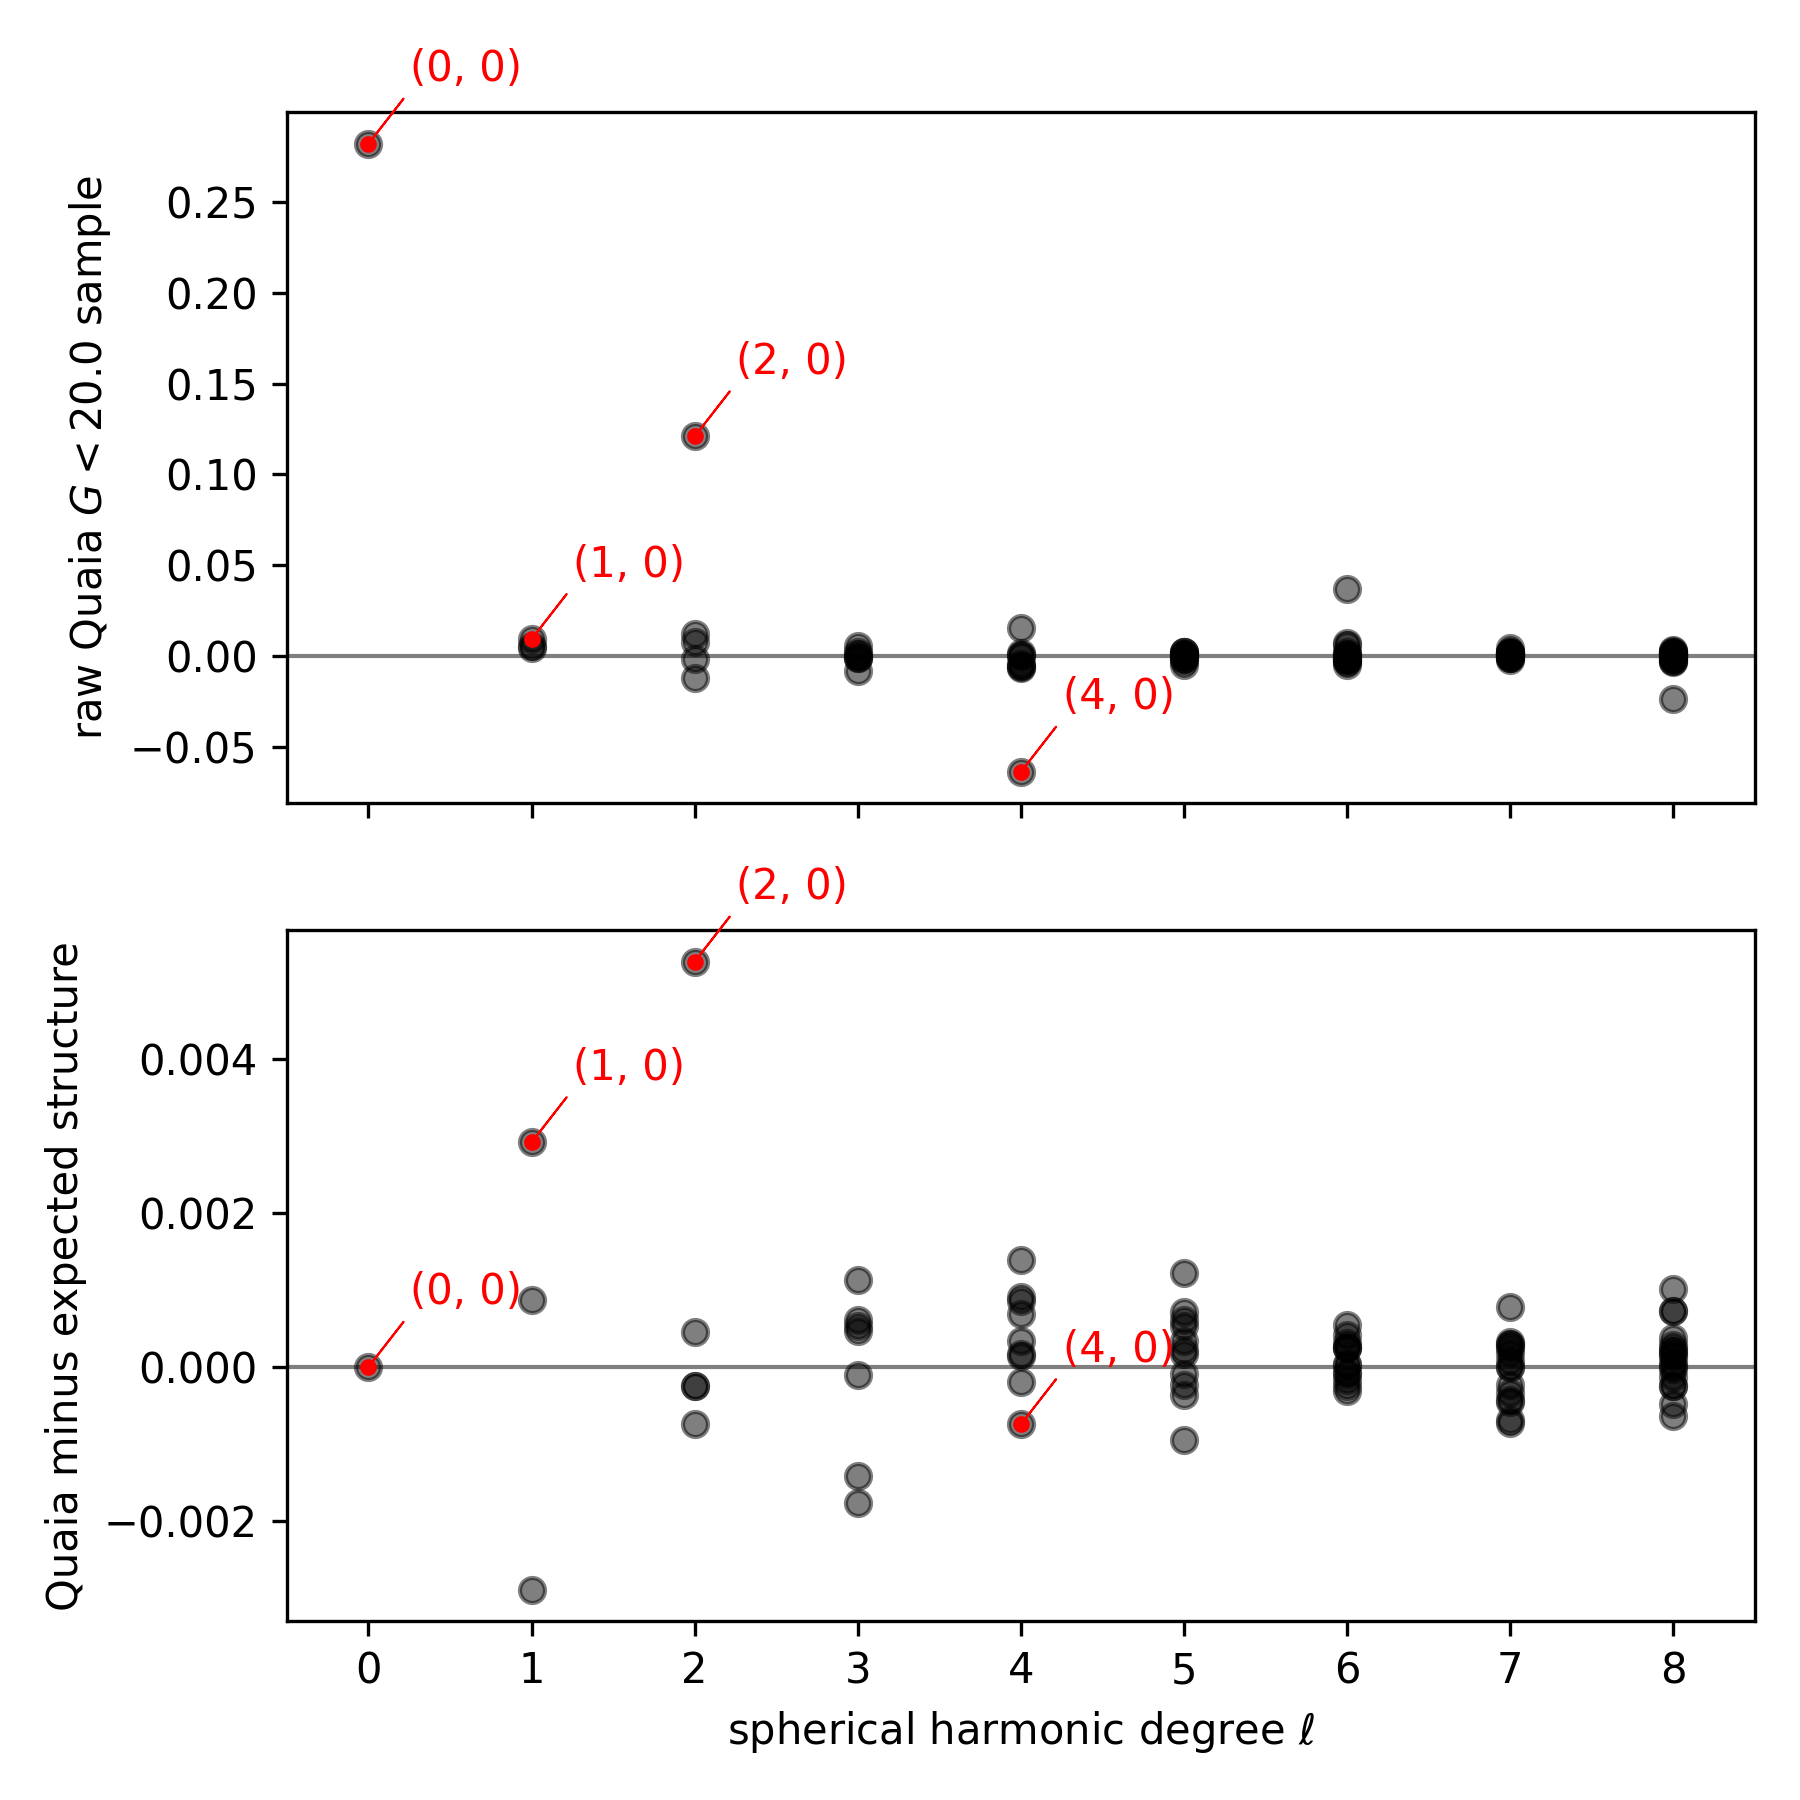
\includegraphics[width=\figurewidth]{notebooks/alms.png}
  \end{center}
    \caption{The spherical-harmonic expansion for the sky distribution, in the natural Galactic coordinate-system spherical harmonics. \textsl{Top:} The real and imaginary amplitudes of the spherical-harmonic expansion for the data set. It has a large amplitude at $(\ell,m)=(2,0)$ because of the quadrupolar form of the extinction map (and therefore sample selection). \textsl{Bottom:} The same, but the real and imaginary amplitudes for $\ell>0$ have been adjusted for their expectation under the selection function, as it has been represented by the random catalog. The low amplitudes at $\ell>0$ demonstrates the isotropy of the sample. There are still residual amplitudes at $(\ell, m)=(1,0)$, $(2,0)$, and $(4,0)$ as expected if there are small issues with the completeness model (selection function model), which is based on an extinction map and a stellar-density map.\label{fig:alms}}
  \end{mdframed}
\end{figure}
There is clear anisotropy visible in \figref{fig:alms}, in the form of non-zero amplitudes at $\ell>0$.
However, the anisotropic structure can be explained by the selection function.
The bottom panel of \figref{fig:alms} shows the amplitudes again, but after the $\ell>0$ amplitudes have had their expectations, based on the same projection but of the random catalog, subtracted.

In detail, the selection function was inferred (and the random catalog was made) under the assumption that the quasar sample is isotropic (see \citealt{ksf} for details).
Does this make the test shown in \figref{fig:alms} circular or true by assumption?
It does not, because the only freedoms permitted in constructing the random catalog were dependences on observed extinction (according to the infrared-emission map of \citealt{sfd}) and the stellar density (according to a count of stars in the \textsl{Gaia} catalog).
And, indeed, the biggest anisotropic amplitudes are at $(\ell,m)=(1,0)$, $(2,0)$, and $(4,0)$, which are exactly what are expected if this completeness map is not perfect:
The dust extinction map and the stellar extinction map have most of their power in these modes (because we live in a disk Galaxy but do not live at its Center).

\begin{figure}[t!]
  \begin{mdframed}
  \color{captiongray}
  \begin{center}
    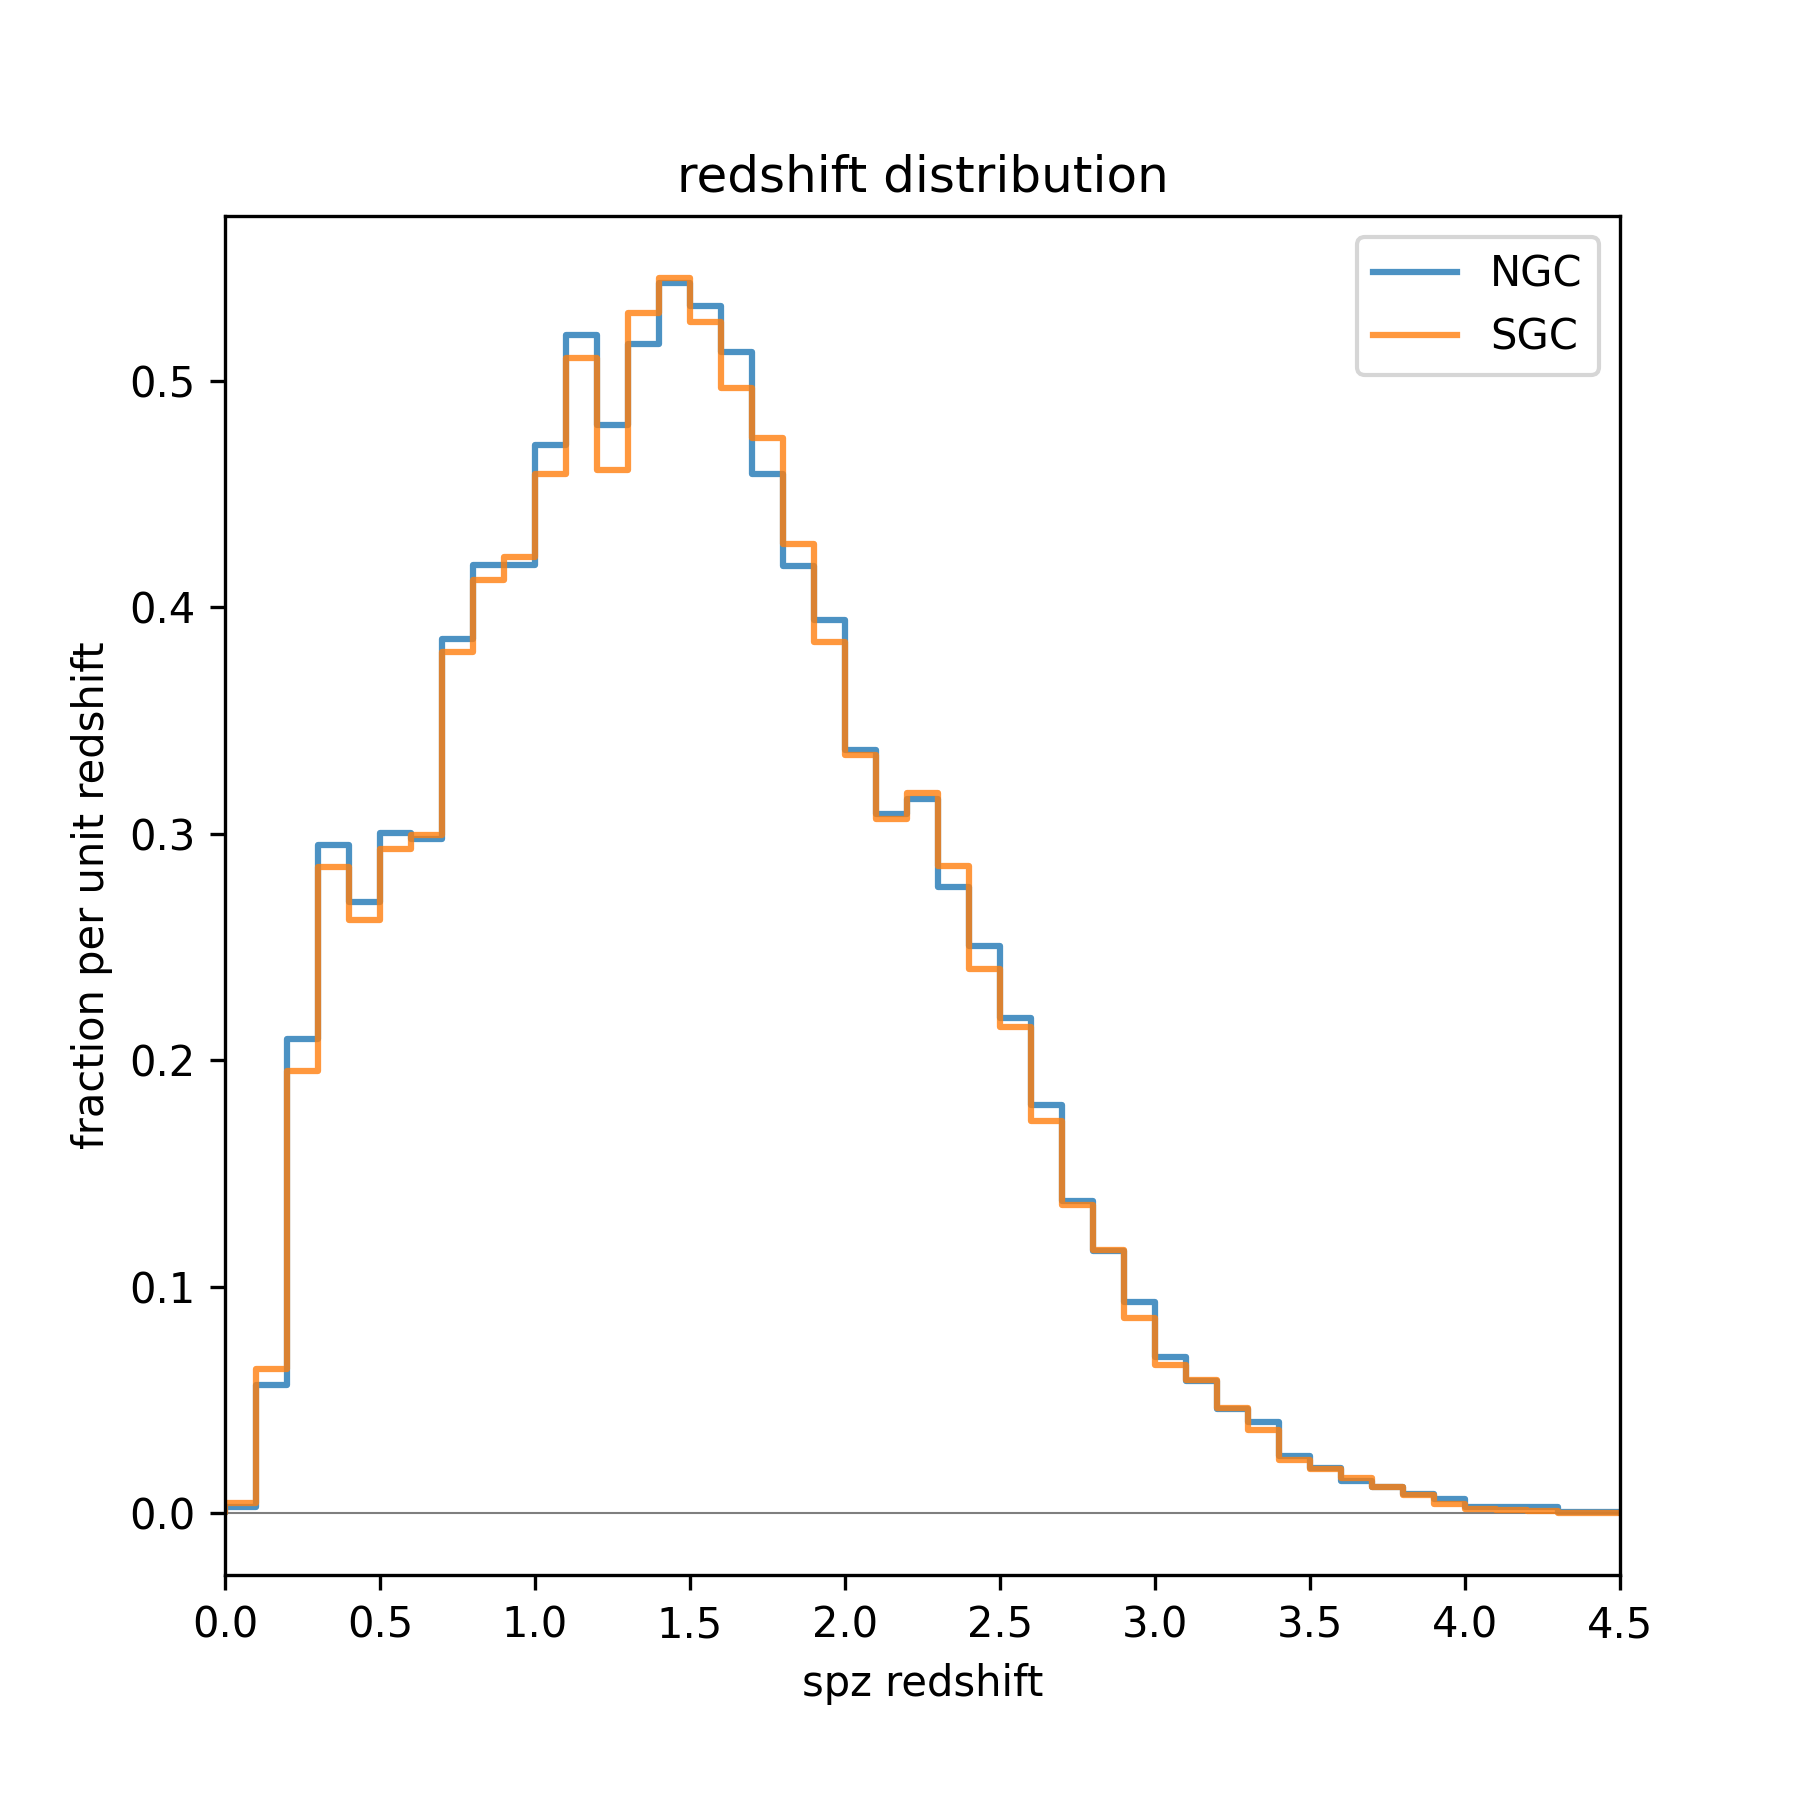
\includegraphics[width=\figurewidth]{notebooks/zhist.png}
  \end{center}
    \caption{The redshift distributions of the NGC and SGC subsamples. This demonstrates that the distribution of quasar spectrophotometric properties is very similar between the North and South.\label{fig:zhist}}
  \end{mdframed}
\end{figure}
Another strong test of isotropy can be obtained from the redshift distribution.
Why is this strong?
It also connects to the hemispherical power asymmetry in the CMB.

In principle we could do something that is even more extreme, which would be the projection of the redshift distribution onto spherical harmonics. Anyone up for that? Might discover non-seperability of the angular and redshift distributions.

\section{Homogeneity}

The weakest possible prediction of homogeneity is that there should be a mean density to the Universe.
This prediction can be cast in terms of the scaling of pair counts or a measurement of the fractal dimension.
The fractal dimension, for a set of points in a space, is defined to be the scaling of the total number of pairs $N$ in the set with the maximum separation $D$ out to which pairs are counted.
If $N$ is proportional to $D^3$ then the fractal dimension is 3 and the Universe has a mean density.

\begin{figure}[t!]
  \begin{mdframed}
  \color{captiongray}
  \begin{center}
    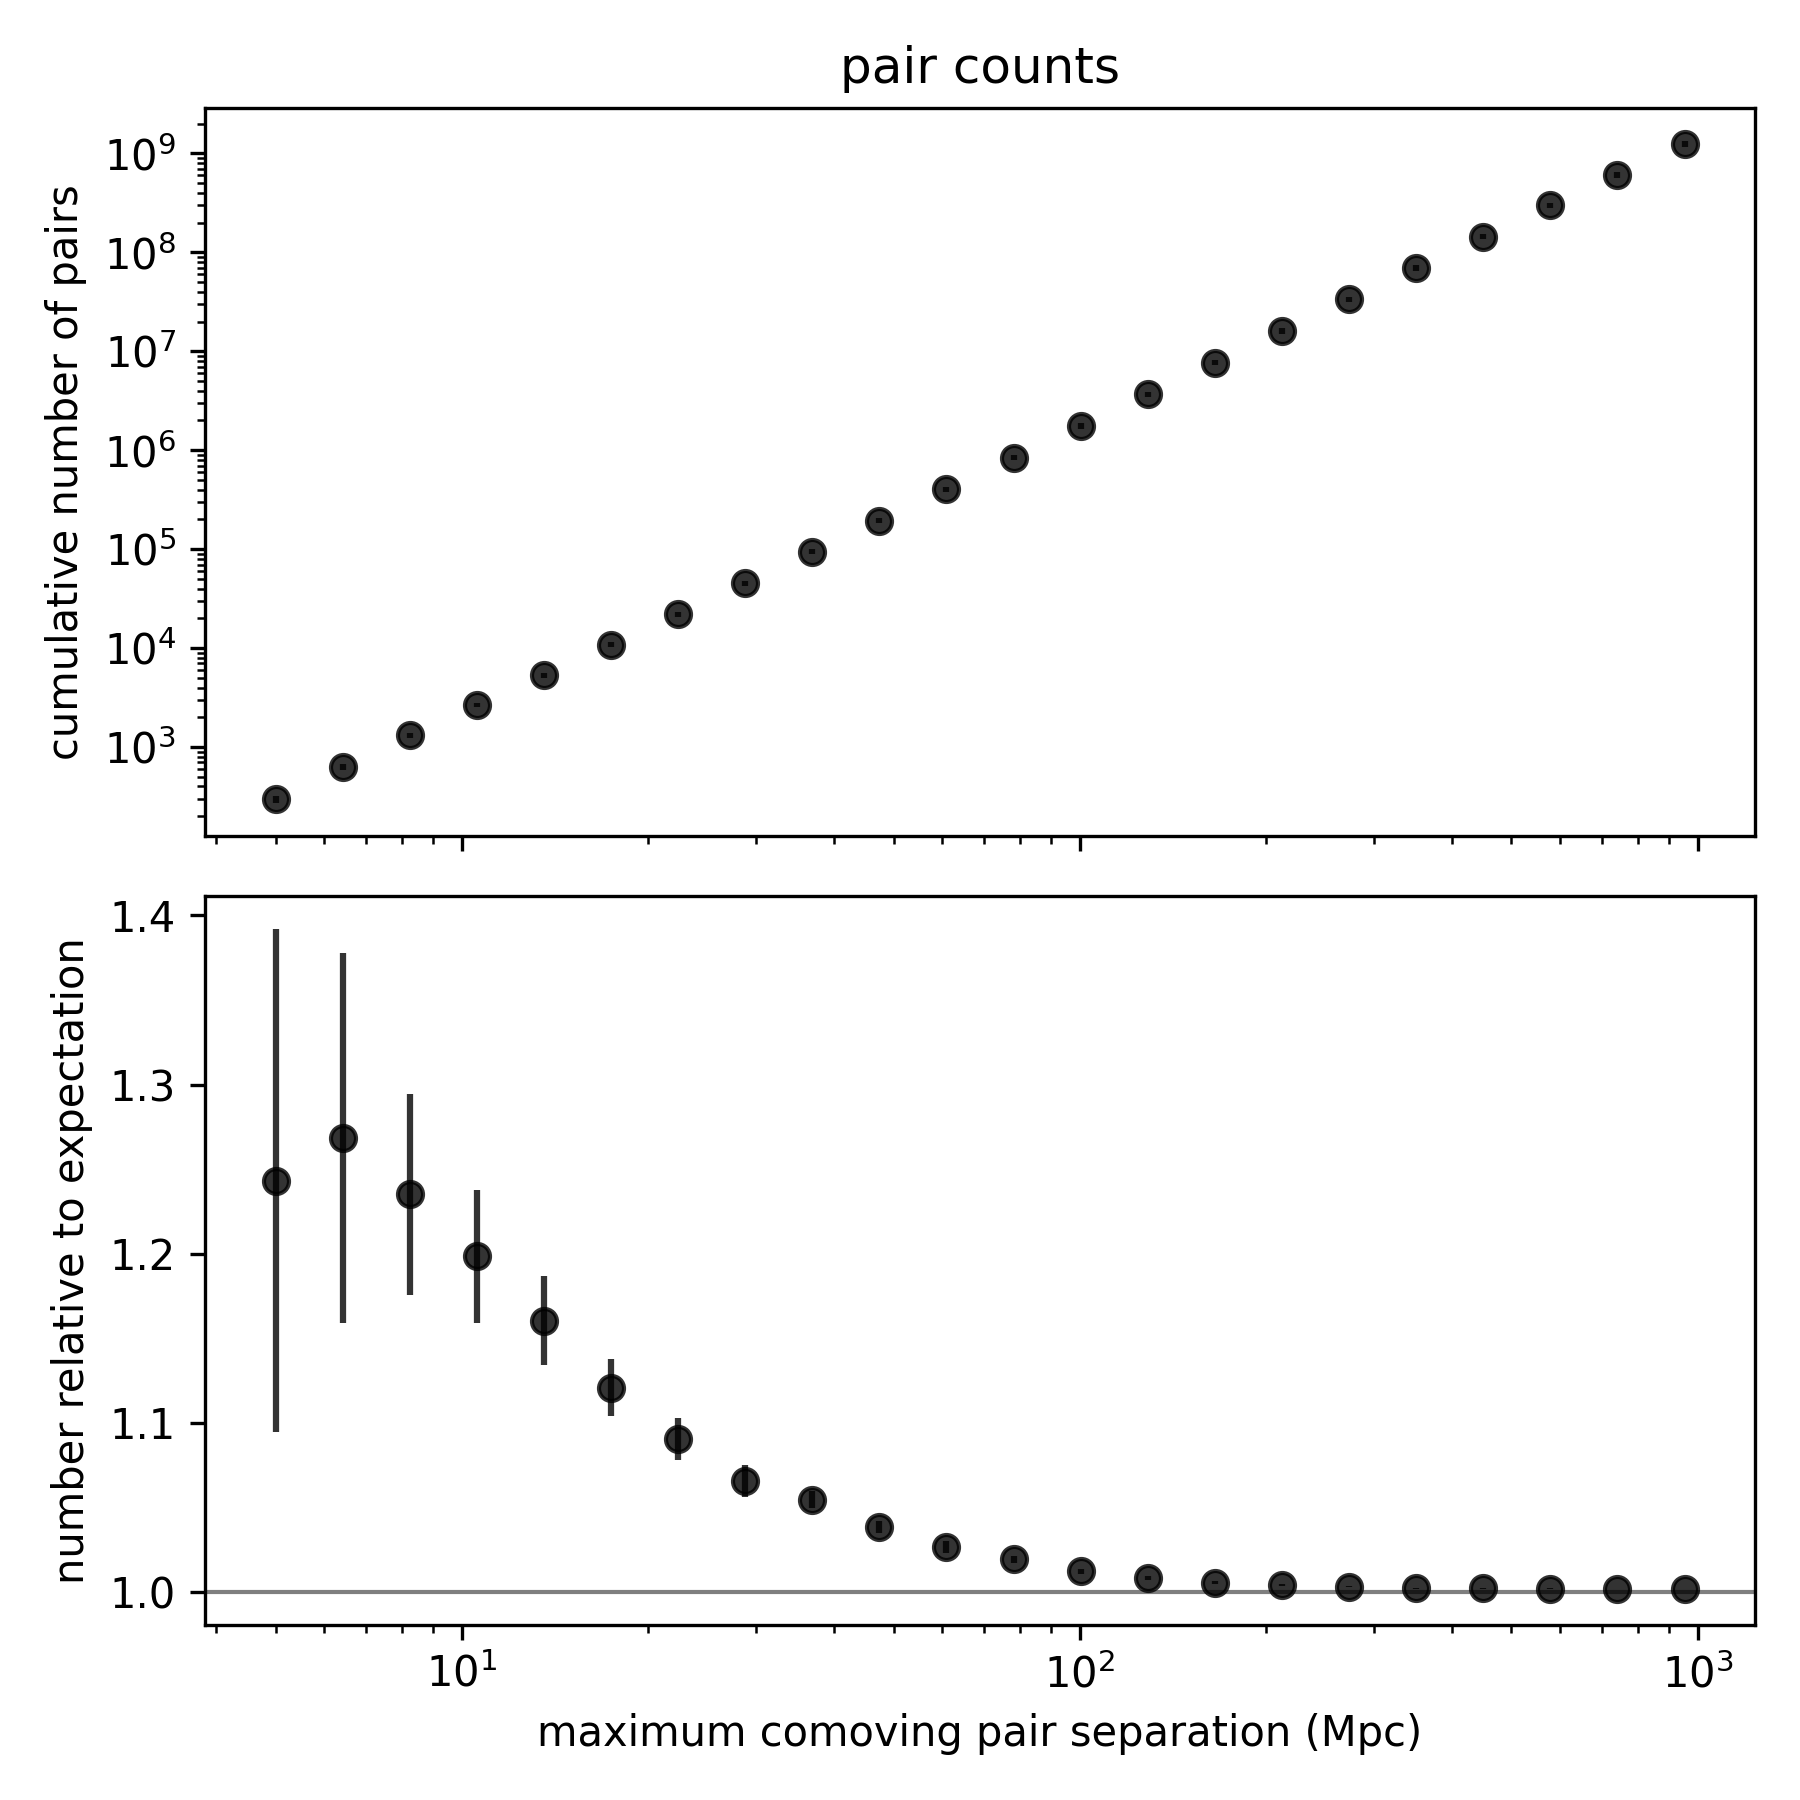
\includegraphics[width=\figurewidth]{notebooks/cumulativeDD_DR.png}
  \end{center}
    \caption{\textsl{Top:} The cumulative total number of quasar--quasar pairs as a function of separation for the NGC and SGC subsamples. Jackknife uncertainty estimates are shown but are smaller than the points for all points.
    \textsl{Bottom:} The same, but divided by the expectation in a homogeneous universe.
    In this case the expectation is estimated with $DR + RD - RR$ (see text for explanation).
    This figure demonstrates that the fractal dimension is extremely close to $3$.\label{fig:cumulative}}
  \end{mdframed}
\end{figure}
The cumulative number of pairs up to separation $D$ is shown as a function of $D$ in \figref{fig:cumulative}.
The top panel shows the raw counts of pairs, and the bottom panel shows the pairs relative to an expectation derived from the random catalog, which (by construction) has fractal dimension $D=3$.
HOGG: EXPLAIN THE EXPECTATION.
HOGG: In detail... Explain the exact nature of the count in terms of what is counted against what.
\figref{fig:cumulative} strongly suggests that the fractal dimension $D$ is 3.
Our best-fit value is ... WHAT?

\section{Statistical isotropy}

If the fractal dimension is 3, then the correlation function should go to zero at large scales.
It does!
But the power asymmetry between the hemispheres challenges \emph{statistical isotropy} which is yet another test.

\begin{figure}[t!]
  \begin{mdframed}
  \color{captiongray}
  \begin{center}
    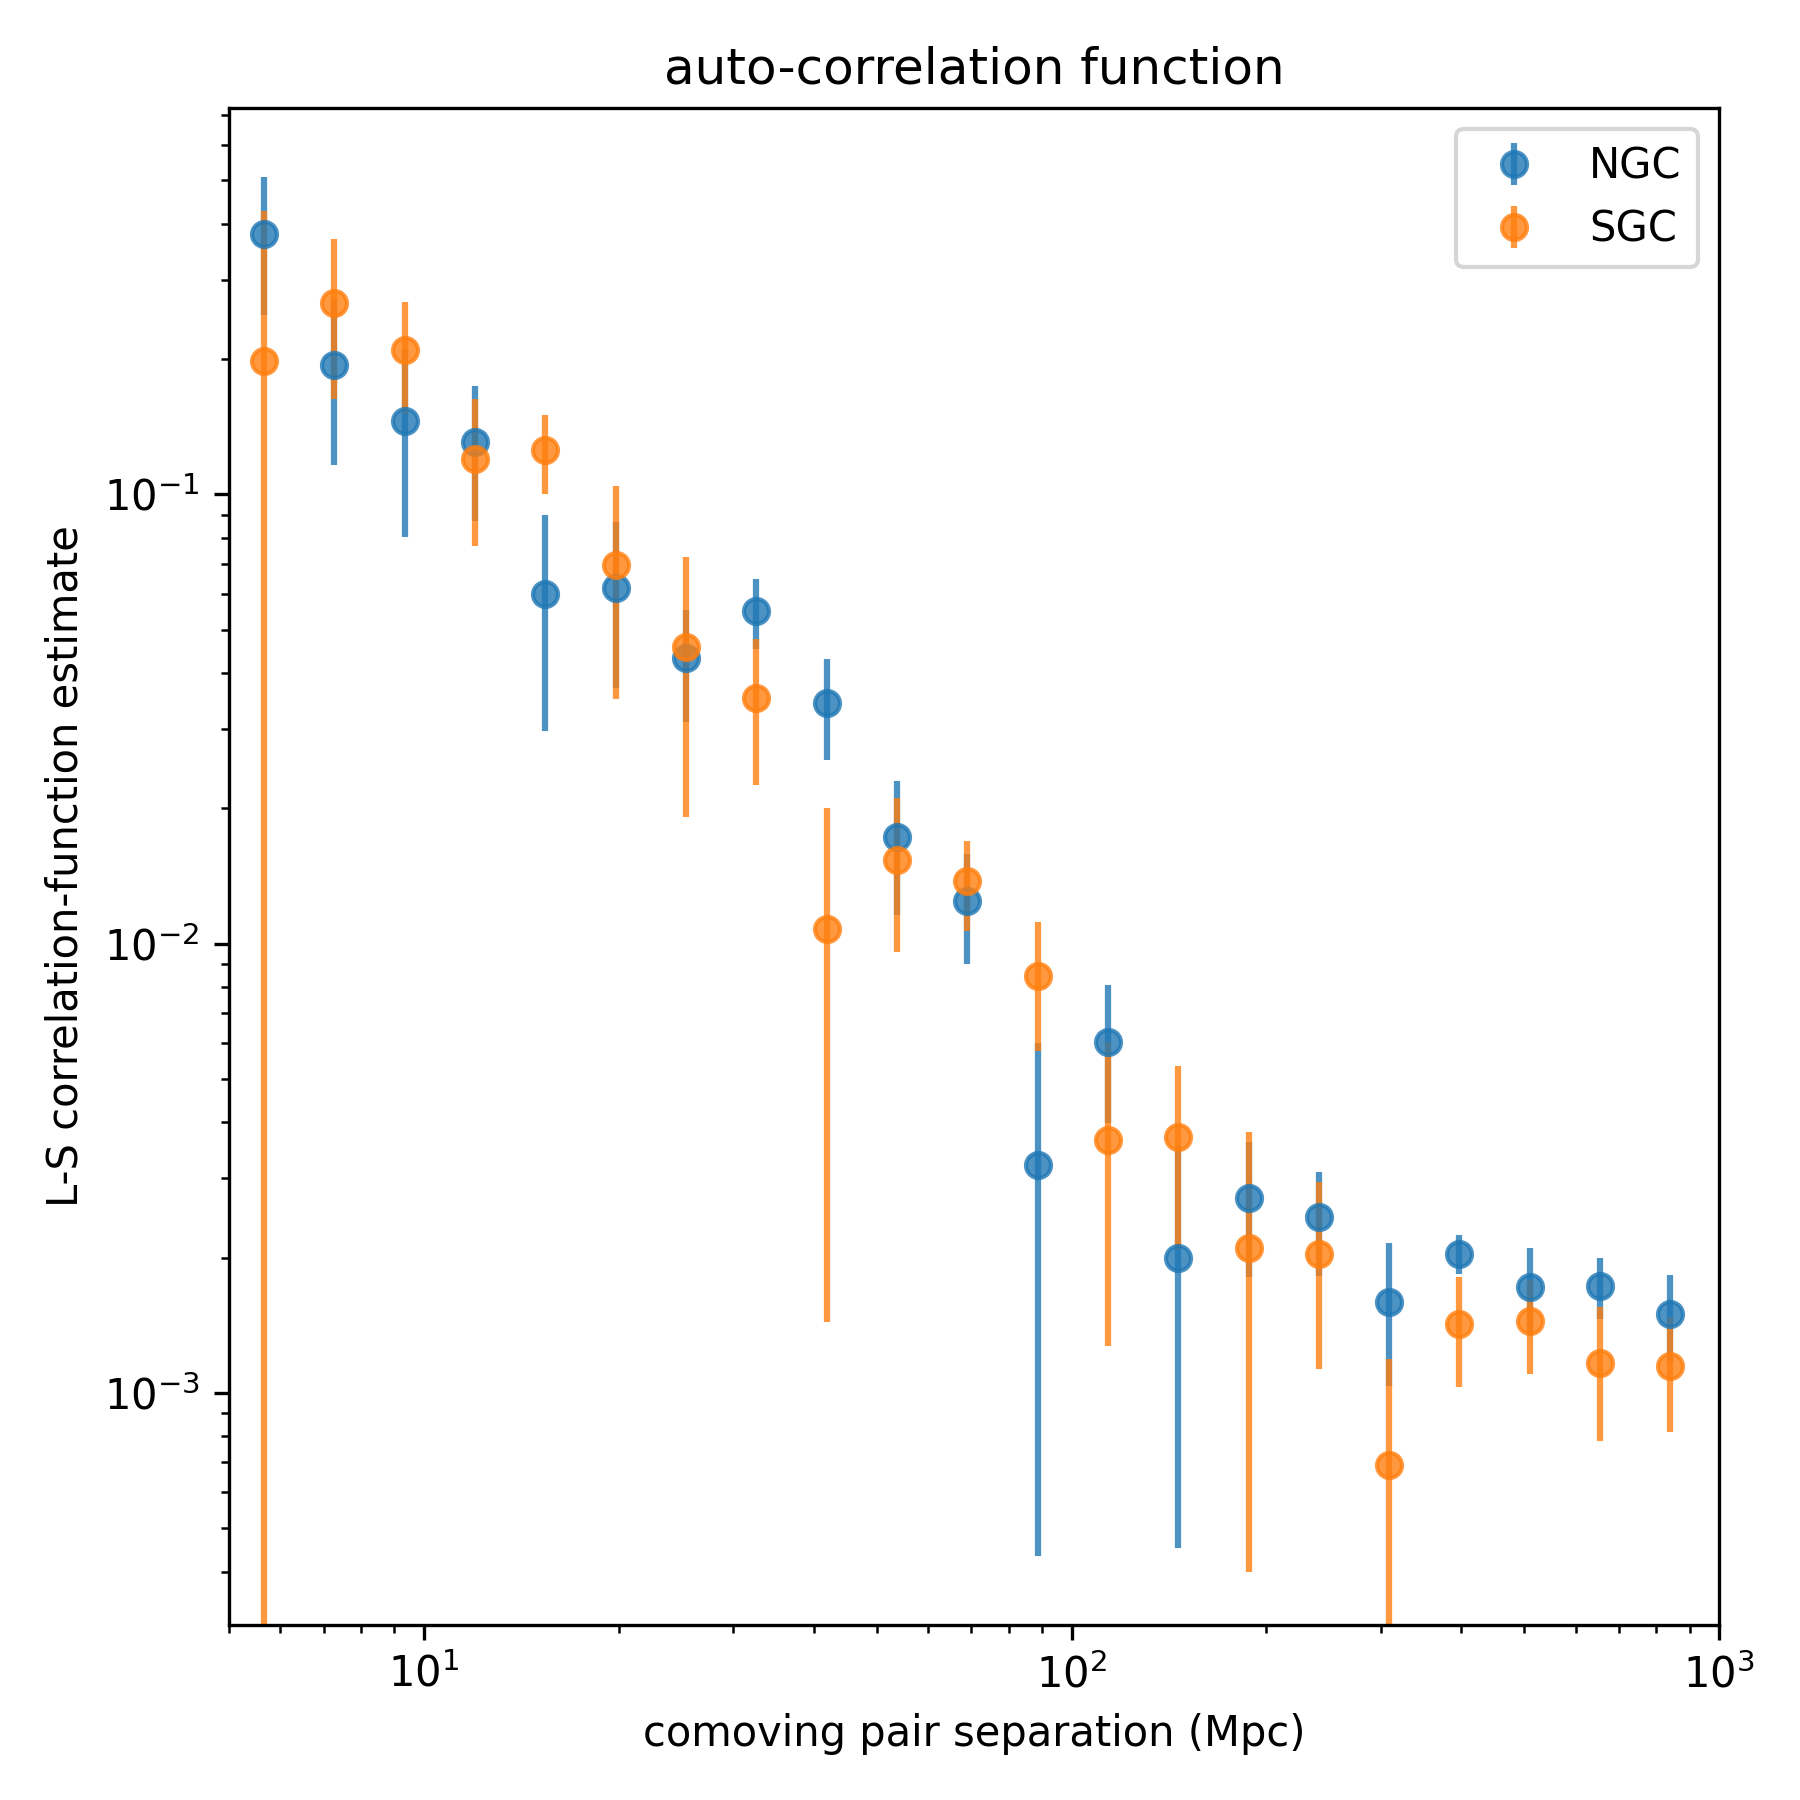
\includegraphics[width=\figurewidth]{notebooks/corrfunc.png}
  \end{center}
    \caption{The auto-correlation of the quasars as a function of separation for the NGC and SGC subsamples.
    This figure demonstrates that the clustering amplitude is similar between the North and the South.\label{fig:corrfunc}}
  \end{mdframed}
\end{figure}

\section{Discussion}

We found what we expected to find, but at very good precision.

How to summarize these results?

ESA \textsl{Gaia} rocks!

\begin{acknowledgements}
Be sure to cite all software: numpy, scipy, matplotlib, astropy.

Be sure to thank the Gaia~F\^ete and Gaia~Hike.

Be sure to put in the full Gaia acknowlegement.

Did we use 2MASS? If so, fix the text to capture it above and below.
\end{acknowledgements}

\facilities{%
European Space Agency (ESA) Gaia Satellite Mission,
NASA 0.4m Wide-field Infrared Survey Explorer (WISE) Satellite Mission,
2.5m Sloan Digital Sky Survey (SDSS) Telescope at Apache Point Observatory (APO)}

\software{%
numpy (\citealt{numpy}),
scipy (\citealt{scipy}),
matplotlib (\citealt{matplotlib}),
astropy (\citealt{astropy})}

\begin{thebibliography}{dummy}
\bibitem[Hoffleit \& Jaschek(1991)]{bsc}
Hoffleit, D. \& Jaschek, C.\ 1991, The Bright Star Catalog. New Haven: Yale University Observatory, 5th rev. ed.
\bibitem[Schlegel et al.(1998)]{sfd} Schlegel, D.~J., Finkbeiner, D.~P., \& Davis, M.\ 1998, \apj, 500, 525. doi:10.1086/305772
\end{thebibliography}

\end{document}
